\apendice{Documento de diseño del juego}

\section{Introducción}
\subsection{Plataforma:}
Ordenador

\subsection{Versión:}
1.0

\subsection{Jugabilidad y contenido:}
El juego consistirá en una serie de niveles independientes que el jugador tendrá que atravesar hasta llegar a la zona de victoria del nivel. Los niveles tendrán una serie de elementos y mecánicas con los que el jugador habrá de interactuar para llegar a la zona de victoria, evitando a distintos obstáculos que pueden truncar la labor del jugador de llegar a la meta.

En el juego habrá un menú principal que permitirá acceder a todos los niveles jugables. Al alcanzar la meta del nivel se volverá al menú principal.

Debido a que la historia no es competencia del TFG, el juego no tendrá historia.

\subsection{Categoría:}
Plataformas 2D

\subsection{Mecánica:}
El jugador manejará un avatar virtual en una serie de niveles de plataformas en los que tratará de llegar a la zona de victoria del nivel utilizando distintas mecánicas de “viajes en el tiempo” y manipulación gravitatoria.

El jugador puede realizar las siguientes acciones:
\begin{itemize}
\item
Moverse.
\item
Saltar.
\item
Realizar un acelerón en una dirección.
\end{itemize}
Las distintas mecánicas con las que puede interactuar el jugador son:
\begin{itemize}
\item
Un portal que teletransportará al jugador de un punto a otro del nivel.
\item
Un creador de impulso que empujará al jugador en un dirección determinada. Esta mecánica se puede manifestar de distintas formas, como una plataforma de salto o una elemento del nivel que escala la velocidad que lleva el jugador.
\item
Tiempo bala, que ralentiza o acelera el tiempo de uno o más elementos del nivel, haciendo que se muevan más rápido o más lento.
\item
Modificadores de la gravedad que influyen en como la gravedad afecta al elemento del nivel al que afecta.
\end{itemize}

\subsection{Tecnología:}
El juego es desarrollado en Unity, utilizando el lenguaje de programación C\#.

\subsection{Visión general del juego:}
El juego consiste en un plataformas 2D de viajes en el tiempo en el que el jugador atravesará una serie de niveles en los que el jugador hará uso de varias mecánicas que influirán en el espacio, el tiempo y la gravedad para esquivar los obstáculos que se interpongan en el camino del jugador y alcanzar la zona de victoria. 

\section{Mecánicas del juego}
\subsection{Jugador}
El jugador controlará un avatar que es capaz de moverse hacia la derecha e izquierda. También puede saltar. El salto es uniforme, se salta cada vez que se pulsa el botón de saltar (espacio en teclado y botón X en el mando) y salta la misma distancia siempre (la fuerza del salto no varía en función de cuánto tiempo se mantenga pulsado el botón de salto). 

Si el jugador colisiona con un obstáculo que le haga daño, el jugador morirá y reaparecerá en la zona inicial del nivel.

El jugador además tiene la habilidad de dar un acelerón hacia la izquierda o la derecha. Este acelerón se realiza en una dirección horizontal, sin variar la posición vertical. Si el acelerón te desplaza X unidades hacia la derecha y está en el punto (1,1) el jugador acabará el acelerón en la posición (1, 1+X). El acelerón lo puedes hacer una sola vez mientras estés en el aire, y en cuanto toques el suelo puedes volver a utilizarlo. En el suelo puedes hacerlo ilimitadamente. Parte de la gracia de este acelerón, es que después de terminarlo sigues manteniendo la velocidad que llevabas durante el acelerón, ahora sí, variando esta según las leyes que rigen el videojuego.

La última herramienta con la que contará el jugador es el tiempo bala. Esta mecánica permitirá reducir la velocidad a la que pasa el tiempo en el nivel permitiendo al jugador actuar con la precisión que ofrece que todo el nivel se reproduzca menor velocidad.

\subsection{Enemigos}
En principio no habrá enemigos vivos como tales. Sin embargo, sí que habrá obstáculos en el juego que, al tocarlos, mataran al jugador. Estos obstáculos pueden ser estáticos o móviles. Los enemigos estáticos no se mueven y la única dificultad radica en evitar colisionar con él. Los obstáculos móviles, sin embargo, pueden ser de dos tipos.

El primer tipo será un obstáculo que aparece en un extremo de la pantalla y se dirige al otro en línea recta. Son obstáculos fáciles de esquivar y predecibles. La dificultad de estos obstáculos radica en lo complejo que puede resultar enfrentarse a varios de ellos y la complejidad improvisada que puede surgir al añadir el obstáculo móvil a un escenario complejo ya de por sí.

El segundo tipo de obstáculo móvil será un obstáculo que se limite a una zona del nivel, pero que siga una rutina de movimiento en esa zona. El riesgo de este obstáculo se limita a una zona reducida del nivel, pero dentro de esta zona el jugador correrá serio riesgo de ser asesinado por el obstáculo.

\subsection{Portal}
Los portales son dos elementos enlazados que parten del hecho de que si entras por un portal tu posición (en ese momento la del portal que has atravesado) se convertirá en la posición del portal pareja del portal por el que has salido. Esta mecánica es sencilla y para nada innovadora, pero que funciona muy bien. Un portal teletransportador es una idea sencilla de utilizar y entender por el jugador.

La gracia de los portales está en salir del segundo portal. Cuando sales del segundo portal, el jugador mantiene la velocidad con la que entró por el primer portal. Esto convierte al hecho de salir por un portal en una mecánica muy variada (y con posibilidades potencialmente infinitas) y que puede dar lugar a puzles interesantes.

\subsection{Creador de impulso}
Esta mecánica consistirá en influir sobre la dirección de la velocidad que lleva un elemento afectado por físicas. Esta mecánica se puede manifestar de distintas formas:
\begin{itemize}
\item
Partícula de impulso: Consiste en un elemento estático en el mapa. Cuando el elemento afectado por las físicas entre en contacto con esta partícula de impulso, este saldrá disparado en una dirección predefinida. La dirección en la que sale disparado el elemento afectado por las físicas será siempre la misma. Eso sí, la dirección es individual para cada partícula, siendo que la partícula siempre dispara el elemento afectado por físicas en una dirección concreta, pero que no tiene por qué ser la misma para dos partículas distintas.
\item
Amplificador de impulso: Consiste en un elemento estático, al igual que la partícula, pero con un funcionamiento ligeramente distinto. Cuando el elemento afectado por físicas entra en contacto con el amplificador, la velocidad que lleva el elemento afectado por físicas se verá escalada. Dos ejemplos de amplificador serían: amplificador positivo de impulso (velocidad = velocidad * X) y amplificador negativo de impulso (velocidad = velocidad/X). Los amplificadores tendrán cada uno un valor particular de escalado del impulso que no tiene por qué coincidir con el resto de amplificadores de impulso.
\item
Plataforma de salto: La típica plataforma de salto que propulsa al jugador cuando entra en contacto con esta. Puede no parecer un elemento creador de impulso, y puede que no lo sea, pero como su funcionamiento es igual al de un creador de impulso, se considera un creador de impulso.
\end{itemize}

\subsection{Modificadores de gravedad}
Elementos que afectan a cómo influye la gravedad sobre uno o varios elemento afectado por físicas. Hay dos tipos de modificadores de gravedad en el juego:

Inversor de gravedad: Elemento estático que provoca que la gravedad se invierta. Esta inversión es “absoluta” en el sentido de que invertir una gravedad de -9,81 hace que esta se convierta en 9,81. Pero una gravedad de -8 invertida la convierte en 8 y no en 9,81.

Obstáculos superdensos: Estos son un tipo especial de enemigo, que, a su alrededor, generan un capo gravitatorio que empuja a los elementos afectados por físicas hacia ellos. Estos obstáculos tienen que luchar por la gravedad que afecta a los elementos afectados por físicas. Como ejemplo, si un elemento afectado por físicas se ve afectado por una gravedad de (-9.81, 0) y un obstáculo con una gravedad (5, 0) el elemento afectado por físicas, en caso de estar debajo del obstáculo verá su gravedad será convertida a (-4,81, 0), pero si el elemento afectado por físicas esta encima del obstáculo su gravedad será convertida a (-13.81, 0).

Esta es una explicación rápida para que se entienda, pero también afectará al elemento afectado por físicas la distancia a la que se encuentre del obstáculo.

En caso de alcanzar el centro de este obstáculo el elemento afectado por físicas morirá si tiene vida, si no se quedará atrapado en el centro.

\subsection{Tiempo bala}
Esta mecánica se basa en manipular como el tiempo afecta a uno o varios elementos afectados por físicas. Esta mecánica es la más costosa de implementar tanto en tiempo como en esfuerzo. Es por ello que no se va a ser demasiado preciso al respecto, pero en principio, esta mecánica se manifestará de dos formas distintas.

Escalar el tiempo: El jugador podrá pulsar el botón de “Tiempo bala” y reducir el tiempo y como este afecta al entorno. Esta reducción de tiempo será una escala de 1/X veces la influencia que tiene el tiempo sobre los elementos afectados por físicas. Esta mecánica afecta a todos los elementos por igual y la escala será siempre la misma para todo el juego y todos los niveles.

Zonas de tiempo escalado: Son zonas en el nivel que escalan el tiempo de todos los elementos que entren dentro de su área de influencia. La forma en la que escalan el tiempo puede ser positiva (tiempo = tiempo * X) o negativa (tiempo = tiempo/X).

Las zonas de tiempo escalado son estáticas en el mapa y la magnitud en la que escalan el tiempo es particular para cada zona, pudiendo ser distinta del resto de zonas de tiempo escalado.


\section{Niveles}
Habrá tres tipos distintos de niveles:

\subsection{Niveles de prueba}
Estos niveles son inaccesibles para el jugador. Son niveles utilizados por el desarrollador para comprobar el correcto funcionamiento del juego e incluso forzar algunos errores intencionalmente. El uso de estos niveles será exclusivo para el desarrollo del proyecto.

\subsection{Niveles tutorial}
Niveles básicos utilizados para introducir mecánicas al jugador y ayudarles a comprender los conceptos que se le explican en un entorno controlado. Estos niveles pueden coincidir con algún nivel de prueba que resulte conveniente tanto para comprobar el funcionamiento básico de una mecánica como para explicar el funcionamiento de la mecánica.

Como ejemplo se va a poner el nivel de prueba de la mecánica de los portales:

\imagen{Anexos/Anexo_F/Nivel_portales}{Nivel tutorial de los portales}

Este nivel se usa para comprobar el correcto funcionamiento de los portales. Pero adicionalmente introduce una serie de conceptos interesantes de manera sencilla y “natural” que pueden servir como tutorial de esta mecánica al jugador. 

Los conceptos que introduce este nivel y lo hace un buen tutorial es que el jugador no tiene mecánicas ajenas interponiéndose en el tutorial (y las que lo hacen, como el salto, son mecánicas que el jugador ya tiene interiorizado. Otro punto fuerte del nivel reside en que soluciona dudas lógicas al jugador como ¿Cómo puedo saber dónde voy a salir si entro por el portal y cómo diferencio pares de portales? Por último, este nivel no puede ser superado sin hacer uso de la mecánica que se desea explicar.

Esta ejemplificación es importante porque todos los niveles tutorial seguirá (en mayor o menor medida) esta estructura.

\subsection{Niveles}
El tercer tipo de nivel no dice mucho por su nombre, siendo este demasiado general. Esto no es algo malo, ya que este tercer apartado abarca todos los niveles que no tienen un propósito explicito. El objetivo de este nivel es exclusivamente alcanzar la zona de victoria. La dificultad de estos niveles puede ser variable y las mecánicas ser combinadas sin compromiso. 
Evidentemente estos niveles están regidos por algunas limitaciones como no utilizar mecánicas que no hayan sido presentadas en un tutorial o que (preferentemente) la dificultad de los niveles sea mayor en los últimos niveles antes que en los primeros.

\section{Interfaces}
El patrón de pantalla que más se va a repetir será el nivel sin ningún elemento extradiegético que afecte a la pantalla del nivel. No se incluyen elementos HUD (Head-Up Display) que monitoricen la vida ni otros elementos que no se consideren monitorizar, prácticamente por su ausencia (siendo el estado de los elementos variables, se puede saltar o se tiene el acelerón disponible, muy sencillos de mantener en mente).

Va a haber, aun así dos interfaces extra disponibles para el jugador. Al no tener las interfaces todavía desarrolladas se va a añadir a continuación un esquema de cómo serán estas interfaces.

\subsection{Pantalla de elección de nivel}
\imagen{Anexos/Anexo_F/Pantalla_de_elección_de_nivel}{Idea inicial de la pantalla de selección de nivel}

\subsection{Pantalla de opciones}
\imagen{Anexos/Anexo_F/Pnatalla_de_opciones}{Idea inicial de la pantalla de opciones}

Estas pantallas son orientativas y susceptibles de cambios. De la misma forma no se tiene que seguir ciegamente el patrón de colores pero se ha de entender la existencia de un patrón de colores y como este se va a aplicar.

\section{Anexos}
A continuación se incluirá información más concreta al respecto del diseño de juego como sprites e imágenes que identificarán a una mecánica o elemento del juego en los niveles, configuración de los controles y descripción una por una de cada nivel del juego.

\subsection{Elementos}
\subsubsection{Player}
Objeto que controlará el jugador. El jugador tiene la capacidad de hacer que el Player se mueva, salte y pegue acelerones.

El Player se puede morir en caso de que colisione con un objeto que reduzca su vida a 0. El Player tendrá solo 1 punto de vida y cuando colisiones con un objeto que lo “dañe”, su vida se reducirá a 0 y morirá. Cuando el Player muera reaparecerá en un punto de reaparición establecido en la escena.

\begin{figure}[h]
\centering

\includegraphics{Anexos/Anexo_F/Sprite_Player}
\caption{Sprite utilizado para el Player}
\end{figure}
\raggedright
\textit{Los sprites y las animaciones del Player los ofrecía Platformer Microgame para uso libre.}

\subsubsection{Enemigos}
\begin{figure}[h]
\begin{itemize}
\item
Obstáculos: Enemigos que no se mueven. Se encuentran estáticos en un lugar y si el Player los toca este se muere. Puede ser que los obstáculos en vez de estar quietos sigan una ruta prestablecida.
\end{itemize}
\centering
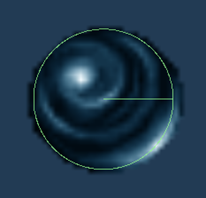
\includegraphics{Anexos/Anexo_F/Obstaculos_estaticos}
\caption{Sprite utilizado para el obstáculo estático}
\raggedright
\textit{El sprite utilizado para los obstáculos pertenece a Daniel Cook y ha sido obtenida en el siguiente enlace: \url{https://opengameart.org/content/iron-plague-teleportbmp}.}
\end{figure}

\begin{figure}[h]
\begin{itemize}
\item
Obstáculos que siguen una rutina: Enemigos que se encuentran en una zona y recorren un camino cíclico continuamente.
\end{itemize}
\centering
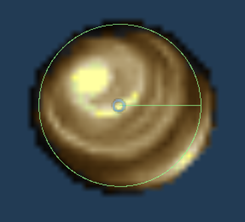
\includegraphics{Anexos/Anexo_F/Obstaculo_en_rutina}
\caption{Sprite utilizado para el obstáculo que sigue una rutina}
\raggedright
\textit{El sprite utilizado para los obstáculos pertenece a Daniel Cook y ha sido obtenida en el siguiente enlace: \url{https://opengameart.org/content/iron-plague-teleportbmp}.}
\end{figure}

\begin{figure}[h]
\begin{itemize}
\item
Obstáculos móviles: Enemigos que aparecen en un extremo de la pantalla y la atraviesa hasta el otro extremo. Si en algún momento el obstáculo móvil toca al Player, este morirá.
\end{itemize}
\centering
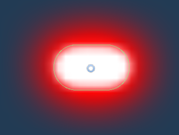
\includegraphics{Anexos/Anexo_F/Obstaculo_movil_rapido}
\caption{Obstáculo móvil rápido}
\end{figure}

\begin{figure}[h]
\centering
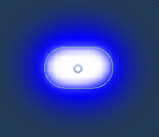
\includegraphics{Anexos/Anexo_F/Obstaculo_movil}
\caption{Obstáculo móvil (velocidad intermedia)}
\end{figure}

\begin{figure}[h]
\centering
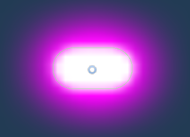
\includegraphics{Anexos/Anexo_F/Obstaculo_movil_lento}
\caption{Obstáculo móvil lento}
\raggedright
\textit{El sprite utilizado para los obstáculos móviles pertenece a Rawdanitsu y ha sido obtenida en el siguiente enlace: \url{https://opengameart.org/content/lasers-and-beams}.}
\end{figure}
\clearpage

\subsubsection{Escenarios}
\begin{itemize}
\item
Suelo
\item
Pared
\item
Zonas de muerte
\item
Zonas de victoria
\end{itemize}

\subsection{Mecánicas}
\subsubsection{Portal}
Portal que teletransporta a los objetos que entren manteniendo la dirección del movimiento del objeto.

\begin{figure}[h]
\centering
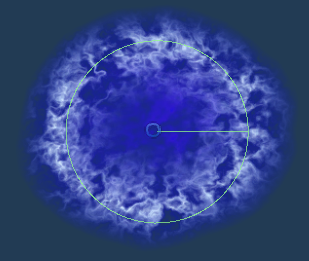
\includegraphics{Anexos/Anexo_F/Portal}
\caption{Sprite utilizado para los portales}
\raggedright
\textit{El sprite utilizado para los portales pertenece a Hansjörg Malthaner y ha sido obtenida en el siguiente enlace: \url{https://opengameart.org/content/animated-portal-or-wormhole-several-variants}.}

\textit{Enlace al trabajo de Hansjörg Malthaner : \url{http://opengameart.org/users/varkalandar}}
\end{figure}

\subsubsection{Creador de impulso}
El objeto afectado recibe un impulso en una dirección.
\begin{figure}[h]
\begin{itemize}
\item
Partícula de impulso: objeto que se encuentra en el escenario. Cuando un objeto toca esa partícula recibe un impulso en la dirección asignada a la partícula.
\end{itemize}
\centering

\includegraphics{Anexos/Anexo_F/Particula_de_impulso}
\caption{Sprite utilizado para la partícula de impulso}
\raggedright
\textit{Los sprites utilizados para la partícula de impulso pertenecen a oglsdl y ha sido obtenida en el siguiente enlace: \url{https://opengameart.org/content/glow-arrow}.}

\textit{El audio utilizado para la partícula de impulso de salto pertenece a Bart Kelsey y ha sido obtenida en el siguiente enlace: \url{https://opengameart.org/content/spell-2}}
\end{figure}

\begin{figure}[h]
\begin{itemize}
\item
Amplificador de impulso: parecido a la partícula de impulso pero escalando el impulso que lleva el objeto.
\end{itemize}
\centering

\includegraphics{Anexos/Anexo_F/Amplificador_de_impulso}
\caption{Sprite utilizado para el amplificador de impulso}
\raggedright
\textit{Los sprites utilizados para el amplificador de impulso son una modificación de un Sprite que pertenece a oglsdl que ha sido obtenida en el siguiente enlace: \url{https://opengameart.org/content/glow-arrow}.}

\textit{El audio utilizado para la partícula de impulso de salto pertenece a Bart Kelsey y ha sido obtenida en el siguiente enlace: \url{https://opengameart.org/content/spell-2}}
\end{figure}

\begin{figure}[h]
\begin{itemize}
\item
Plataforma de salto: Se define por si sola.
\end{itemize}
\centering

\includegraphics{Anexos/Anexo_F/Plataforma_de_salto}
\caption{Sprite utilizado para el amplificador de impulso}
\raggedright
\textit{Los sprites utilizados para la plataforma de salto pertenecen a diana23570 y ha sido obtenida en el siguiente enlace: \url{https://opengameart.org/content/spring}.}

\textit{El audio utilizado para la plataforma de salto pertenece a Blender Foundation y ha sido obtenida en el siguiente enlace:  \url{https://opengameart.org/content/sprint-jumpinteraction-sound-yo-frankie}}
\end{figure}

\clearpage
\subsubsection{Tiempo bala}
Capacidad de “ralentizar o acelerar el tiempo” influyendo en la velocidad a la que afecta al uno o varios objetos que se ven afectados. Esta mecánica se manifiesta escalando las físicas de los objetos afectados.
\begin{itemize}
\item
Escalar el tiempo: Capacidad del Player para escalar el tiempo que afecta a todos los objeto.
\item
Zonas de tiempo escalado: Zonas que escalan el tiempo de los objetos que entran en la zona de influencia de la zona.
\end{itemize}

\begin{figure}[h]
\centering
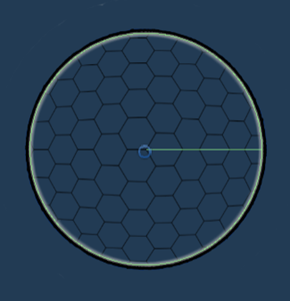
\includegraphics{Anexos/Anexo_F/Zonas_tiempo_escalado}
\caption{Sprite utilizado para la zona de tiempo escalado}
\raggedright
\textit{El sprite utilizado para las zonas de tiempo escalado es una modificación de un sprote que pertenece a scenna y ha sido obtenida en el siguiente enlace: \url{https://opengameart.org/content/circle}.}
\end{figure}

\subsubsection{Acelerón}
El jugador realiza un acelerón en la dirección en la que está mirando.

\subsubsection{Modificadores de gravedad}
Objetos que afectan a como la gravedad influye sobre ellos u otros objetos.
\begin{figure}[h]
\begin{itemize}
\item
Inversor de gravedad: vuelve la gravedad negativa en positiva y viceversa.
\end{itemize}
\centering

\includegraphics{Anexos/Anexo_F/Inversor_gravedad}
\caption{Sprite utilizado para el inversor de gravedad}
\raggedright
\textit{El sprite utilizado para los inversores de gravedad pertenece a Rawdanitsu y ha sido obtenida en el siguiente enlace: \url{https://opengameart.org/content/lasers-and-beams}.}

\begin{itemize}
\item
Obstáculos superdensos: Obstáculos hacia los que te ves atraído debido a su alta gravedad.
\end{itemize}
\centering
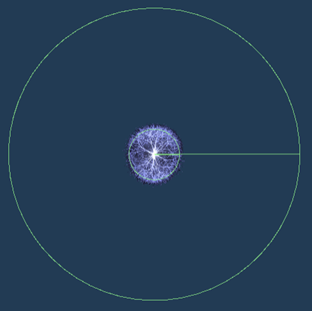
\includegraphics{Anexos/Anexo_F/Obstaculo_superdenso}
\caption{Sprite utilizado para el obstáculo superdenso}
\raggedright
\textit{Los sprites utilizados para la plataforma de salto pertenecen a Hansjörg Malthaner y ha sido obtenida en el siguiente enlace: \url{https://opengameart.org/content/animated-charged-bolt}.}

\textit{Enlace al trabajo de Hansjörg Malthaner: \url{http://opengameart.org/users/varkalandar}}
\end{figure}

\clearpage
\subsection{Controles}
\subsubsection{Mando}
Los controles del mando se regirán por la nomenclatura de los controles de PlayStation.

\begin{figure}[h]
\centering
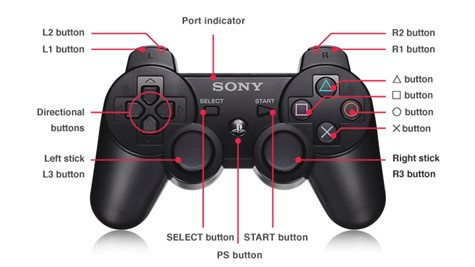
\includegraphics{Anexos/Anexo_F/Mando_play}
\caption{Nomenclatura de los mandos de PlayStation}
\end{figure}

\begin{itemize}
\item
\textbf{Movimiento:} Stick izquierdo.
\item
\textbf{Salto:} botón X (Joystick button 1 en Unity)
\item
\textbf{Acelerón:} botón O (Joystick button 2 en Unity)
\item
\textbf{Tiempo bala:} botón R1 (Joystick button 5 en Unity)
\item
\textbf{Abrir el menú de pausa:} botón R2(Joystick button 7 en Unity)
\end{itemize}

\subsubsection{Teclado}
\begin{itemize}
\item
\textbf{Movimiento:} flecha izquierda para ir a la izquierda y flecha derecha para ir a la derecha.
\item
\textbf{Salto:} espacio 
\item
\textbf{Acelerón:} tecla S
\item
\textbf{Tiempo bala:} tecla D
\item
\textbf{Abrir el menú de pausa:} tecla ESC
\end{itemize}

\subsection{Pantallas}
\begin{figure}[h]
\subsubsection{PruebaPlayerScene}
\centering
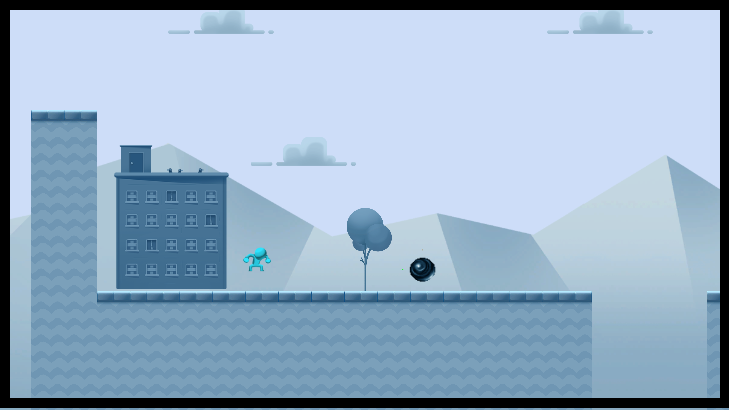
\includegraphics{Anexos/Anexo_F/PruebaPlayerScene}
\caption{Pantalla de prueba de mecánicas básicas }
\end{figure}

\begin{figure}[h]
\subsubsection{PruebaPortalScene}
\centering
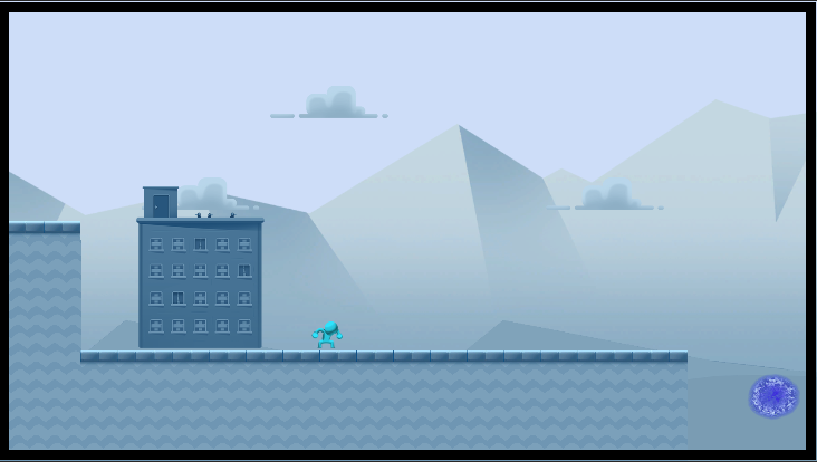
\includegraphics{Anexos/Anexo_F/PruebaPortalScene}
\caption{Pantalla de prueba de los portales }
\end{figure}

\begin{figure}[h]
\subsubsection{PruebaMovingObstacleScene}
\centering
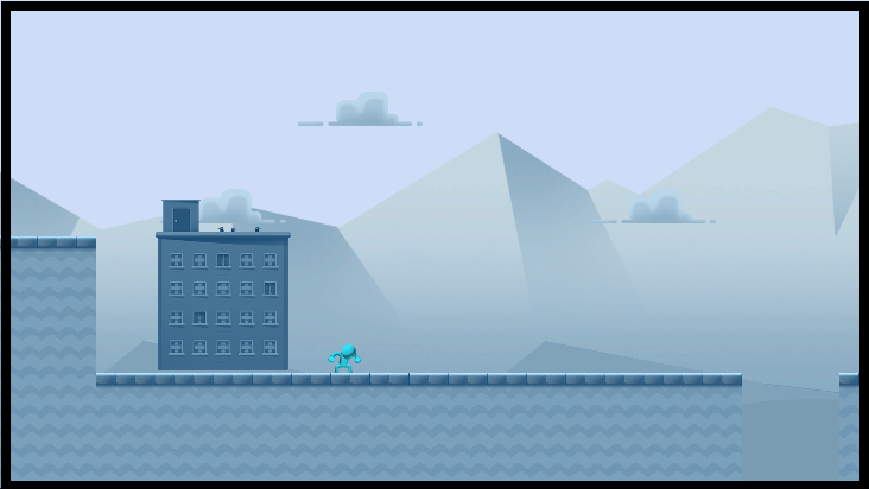
\includegraphics[scale=0.55]{Anexos/Anexo_F/PruebaMovingObstacleScene}
\caption{Pantalla de prueba de los obstáculos móviles }
\end{figure}

\begin{figure}[h]
\subsubsection{PruebaImpulseCreatorsScene}
\centering
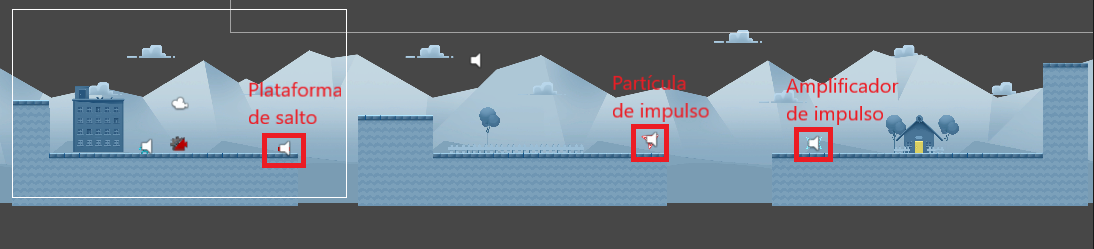
\includegraphics[scale=0.55]{Anexos/Anexo_F/PruebaImpulseCreatorsScene}
\caption{Pantalla de prueba de los creadores de impulso }
\end{figure}

\begin{figure}[h]
\subsubsection{PruebaGravityModifierScene}
\centering
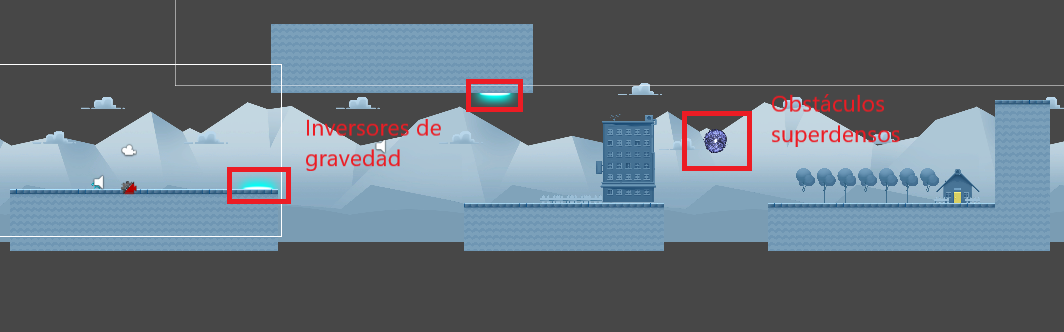
\includegraphics[scale=0.55]{Anexos/Anexo_F/PruebaGravityModifierScene}
\caption{Pantalla de prueba de los modificadores de gravedad }
\end{figure}
\clearpage

\begin{figure}[h]
\subsubsection{PruebaTimeModifierScene}
\centering
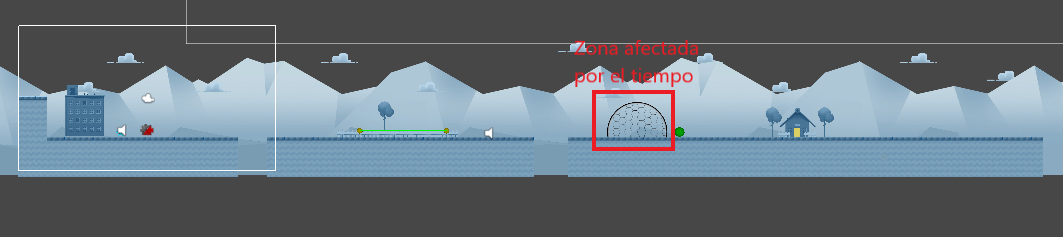
\includegraphics[scale=0.55]{Anexos/Anexo_F/PruebaTimeModifierScene}
\caption{Pantalla de prueba de los modificadores temporales}
\end{figure}